\section{Fremdkapital}

\textbf{Unterschiede Eigenkapital vs. Fremdkapital}:
\begin{center}
	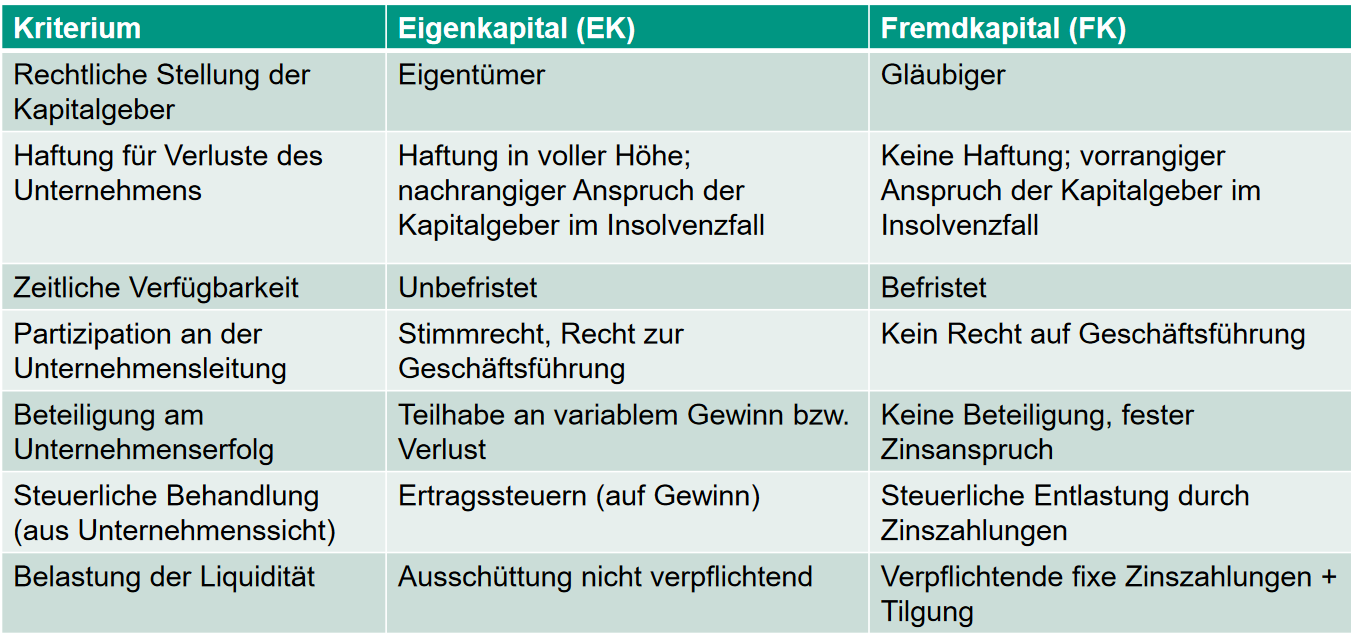
\includegraphics[width=0.8\textwidth]{images/ek-fk.png}
\end{center}

\textbf{Formen des Fremdkapitals}:
\begin{center}
	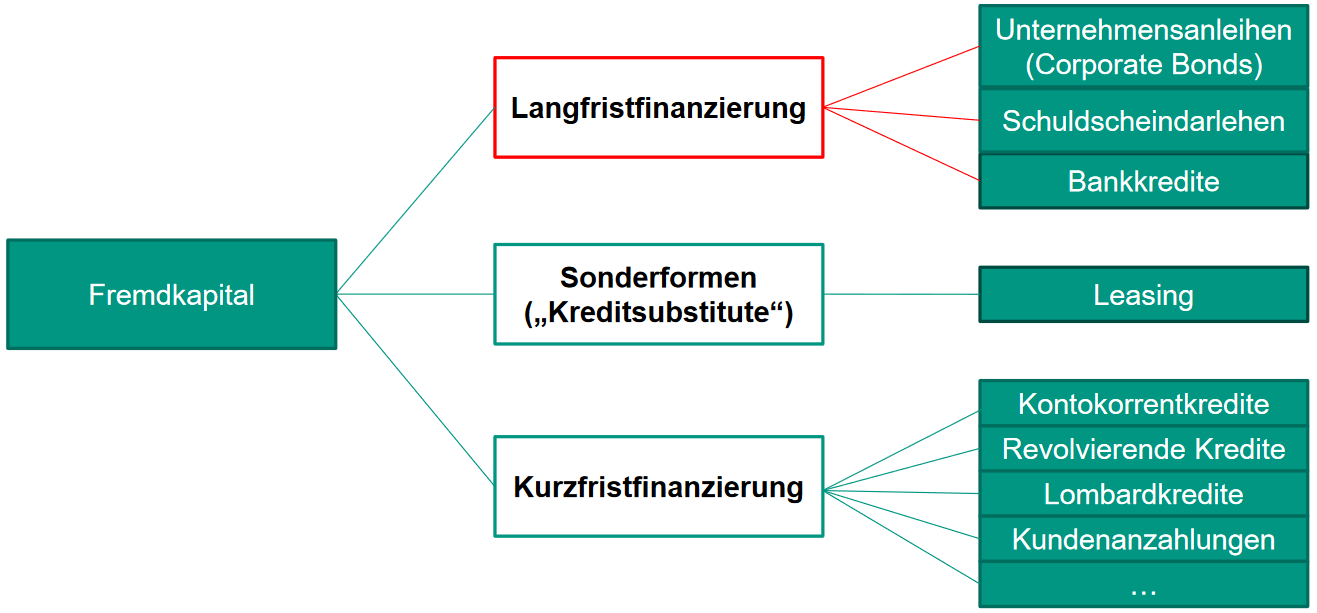
\includegraphics[width=0.6\textwidth]{images/formen-fk.png}
\end{center}

\textbf{Fremdkapitalkosten}: Fremdkapital können wegen den Zahlungsverpflichtungen Zahlungsreihen zugeordnet werden
\begin{center}
	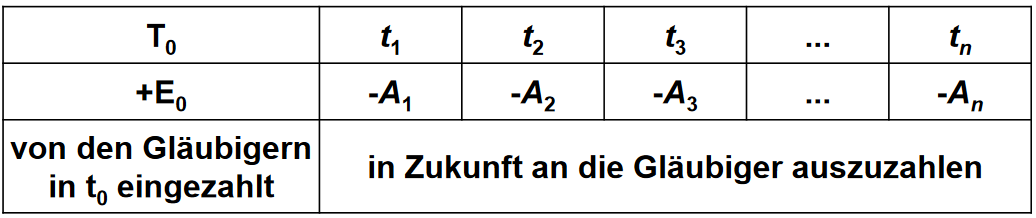
\includegraphics[width=0.5\textwidth]{images/fk-zr.png}
\end{center}
Einzahlungsbetrag $E_0$ von den Gläubigern bestimmt durch:
$$E_0=\sum\limits_{t=1}^{n}\frac{A_t}{(1+i)^t}\qquad\text{mit }i=\text{FK-Kostensatz, ermittelt als interner Zinssatz}$$
$\rightarrow$ Zusätzlich muss das Ausfallrisiko berücksichtigt werden\\

\textbf{Sicheres und unsicheres Fremdkapital}:
\begin{itemize}
	\item \textbf{Sicheres Fremdkapital}: $i$ orientiert sich am risikolosen Zinssatz (z.B. für risikolose Staatsanleihen)
	\item \textbf{Unsicheres Fremdkapital}: $i$ ist die geforderte Rendite der Gläubiger $\rightarrow$ Unterscheiden sich von der erwarteten Rendite, da Risiko übernommen wird
	\item \textbf{Risikoneutrale FK-Geber} fordern einen Zinssatz $i$, um als erwartete Rendite den risikolosen Zins zu erhalten
	\item \textbf{Risikoaverse FK-Geber} verlangen eine zusätzliche Risikoprämie
\end{itemize}
\begin{center}
	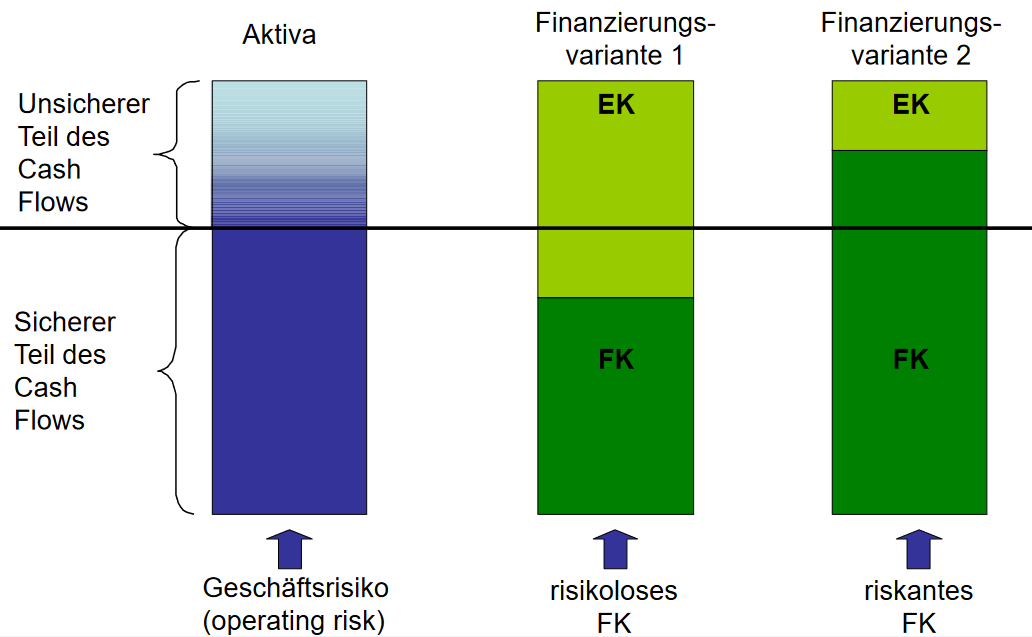
\includegraphics[width=0.6\textwidth]{images/sicher-unsicher.png}
\end{center}

\textbf{Kreditkonditionen}:
\begin{itemize}
	\item Risikofreier Zins als Basisverzinsung
	\item Kompensation für den erwarteten Ausfall (auch bei risikoneutralen FK-Geber)
	\item Risikoprämie (risikoavers)
\end{itemize}
\bigskip
\textbf{Kreditrisiko}: Unterscheidung zwischen:
\begin{itemize}
	\item \textbf{Screening}: Kreditwürdigkeitsprüfung vor Kreditvergabe
	\item \textbf{Monitoring}: Laufende Kreditüberwachung
	
	$\rightarrow$ \textbf{Ziel} der Kreditwürdigkeitsprüfung: Beurteilung der Ausfallwahrscheinlichkeit und die Höhe des Verlustes im Falle eines Ausfalls
	
	\item \textbf{Erwarteter Verlust der Bank}: $$\text{Probability of Default} \cdot \text{Exposure at Default} \cdot \text{Loss Given Default}$$
	\begin{itemize}
		\item Probability of Default: Ausfallwahrscheinlichkeit des Unternehmens
		\item Exposure at Default: Kredithöhe zum Zeitpunkt des Ausfalls
		\item Loss Given Default: Anteil des Kredits der ausfällt
	\end{itemize}
\end{itemize}
\bigskip
\textbf{Credit Rating}: Unabhängige Einschätzung der Fähigkeit eines Kreditnehmers zur termingerechten Erfüllung von Zins- und Tilgungsverpflichtungen

$\rightarrow$ Beeinflussen die Möglichkeit neues Fremdkapital aufzunehmen
$\rightarrow$ Bei schlechten Ratings ist ein Aufschlag zu zahlen

\textbf{Rating Prozess}:
\begin{itemize}
	\item Definition von Kriterien zur Beurteilung der Kreditnehmer
	\item Aggregation der Werte für die einzelnen Kriterien zu einem Score $\rightarrow$ Einteilung in diskrete Rating-Klassen
	\item Schätzung des Zusammenhangs zwischen Score und Ausfallwahrscheinlichkeit unter Verwendung historischer Daten (z.B. Jahresabschlussanalyse)
	\item \textbf{issuer}-specific credit rating: Auf Emittenten bezogen
	\item \textbf{issue}-specific credit rating: Auf emittierte Wertpapiere bezogen
\end{itemize}
\bigskip
\textbf{Jahresabschlussanalyse}: Analyse des vergangenheitsbezogenen Zahlenwerks, um Aussagen über die Zahlungsfähigkeit von Unternehmen gewinnen zu können

\textbf{Kennzahlen}: 
\begin{itemize}
	\item Liquiditätskennzahlen (siehe Kapitel 2)
	\item Verschuldungsgrad (= FK/EK),
	\item Return on Equity (= Gewinn/Buchwert EK),
	\item Anlagendeckungsgrad (= (EK+langfr. FK)/AV),
	\item Zinsdeckungsrate (= EBIT(DA)/Zinsaufwand)
\end{itemize}

\textbf{Z-Score}: Scoring-Verfahren, bei dem eine Auswahl von Bilanzkennzahlen zu einem Score aggregiert wird:
$$\text{Z-Score}=3,25 + 6,56X_1 + 3,26X_2 + 6,72X_3 + 1,05X_4$$
\begin{itemize}
	\item $X_1=$ Net Working Capital/Bilanzsumme
	\item $X_2=$ Einbehaltene Gewinne/Bilanzsumme
	\item $X_3=$ EBIT/Bilanzsumme
	\item $X_4=$ Buchwert des EK/Buchwert der Verbindlichkeiten
\end{itemize}
$\rightarrow$ Je höher der Z-Score, desto verlässlicher\\

\textbf{Debt Tax Shield}: Fremdfinanzierungsbedingte Steuervorteil. Unternehmen zahlen Steuern auf Gewinn nach Abzug von Zinszahlungen $\rightarrow$ Zinsaufwendungen mindern die Höhe der Ertragssteuer
$$\text{Debt Tax Shield}=\text{Ertragssteuersatz}\cdot\text{Zinszahlungen}$$